\documentclass{article}

% Preprint: named authors, no anonymisation.
% For a double-blind workshop submission, swap to:
%   \usepackage[dblblindworkshop]{neurips_2026}
%   \workshoptitle{NAME OF WORKSHOP}
\usepackage[preprint]{neurips_2026}

\usepackage[utf8]{inputenc}
\usepackage[T1]{fontenc}
\usepackage{hyperref}
\usepackage{url}
\usepackage{booktabs}
\usepackage{amsfonts}
\usepackage{amsmath}
\usepackage{nicefrac}
\usepackage{microtype}
\usepackage{xcolor}
\usepackage{graphicx}

\title{Reading Without Looking: Position-Resolved Evidence of\\Visual Bypass in a Small Document OCR Model}

\author{%
  Adya Srivastava\\
  \texttt{srivastavadya@gmail.com}\\
}

\begin{document}

\maketitle

\begin{abstract}
Confidence scores from document OCR models are used to decide which predictions a human
should check. We audit that signal in a small ($\approx$19.6M parameter) encoder--decoder OCR
model trained from scratch with no prior exposure to any Indic script, across three
independently trained seeds. We first establish what the model can do: on held-out real Hindi
scans its grapheme character error rate is 0.985, and on blank white images it is 0.949. The
model does not read real document images, and real and blank input are not distinguishable at
three seeds ($t = 0.257$, $p = 0.822$, 2 df). We then localise the
failure. Under teacher forcing the ground-truth token is never the model's argmax at
generation position~0 (0 of 180 sequences), and the geometric mean probability assigned to the
correct first symbol is $2.2\times10^{-11}$ on real images and $6.3\times10^{-11}$ on blank:
more than eight orders of magnitude below what a text-only $n$-gram model fitted on the same
training corpus, which never sees an image, assigns to that same symbol. Self-generated
max-softmax confidence at that position is nonetheless approximately 0.90. From position~2
to~39 the model recovers to between $-0.15$ and $-0.48$, comparable to a position-matched 4- to
5-gram grapheme prior and near-identical with and without the image; at positions 0, 1 and
beyond 39 it falls far below every $n$-gram baseline. Deleting the encoder changes the
output distribution substantially (mean KL 1.075 nats, argmax flips at 8.2\% of decoding
steps) but leaves its peak near unity: 96.7\% of the divergence sits at those flipped
positions while agreeing positions retain a mean confidence of 0.998. Finally, the confidence signal is not globally broken. On
synthetic in-distribution lines, where the model attains 18.3\% line accuracy, confidence
discriminates correct from incorrect transcriptions at AUROC 0.838 while remaining badly
miscalibrated at a mean of 0.994; on real scans, where accuracy is zero, it carries no usable
correctness signal. We read this as a model whose certainty tracks the linguistic plausibility
of what it generates rather than the state of its own perception. Because visual dependence in
transcription is concentrated at the start of the sequence, a confidence score averaged
uniformly over generated tokens dilutes the one position that carries it; confidence measures
for transcription should weight early positions rather than averaging uniformly.
\end{abstract}

\section{Introduction}

Document OCR is often the first automated step in processing multilingual records, and
production pipelines route low-confidence predictions to human review. The design assumes that
when a model is unsure, it says so.

That assumption is unreliable for large vision--language models. Recent work establishes
\emph{visual ungroundedness}: models produce fluent, confident, sometimes correct output
driven entirely by language priors, with the image contributing nothing, and existing
confidence estimators cannot detect this \citep{khanmohammadi2026bicr}. Related work describes
the same hazard as perception bypass or visual shortcut \citep{xu2026bypass}, and
multilingual OCR benchmarks report that failure on unfamiliar scripts is not silent: models
hallucinate fluent text in familiar scripts rather than abstaining
\citep{kargaran2026glotocr}.

We take that as established and ask a narrower question that autoregressive transcription
makes answerable: \textbf{where in the generated sequence does visual dependence live, and can
its absence be localised without training a probe?}

The question has a structure here that short-answer visual question answering does not offer.
When a decoder transcribes a line token by token, every position after the first can draw on
two sources: the image, through cross-attention, and the preceding tokens, through the
language prior over the training script. These are confounded. Position~0 is not. At
position~0 there is no prefix, so the only \emph{input-dependent} source of information is the
image; whatever the decoder contributes is a fixed marginal over sequence-initial symbols that
cannot vary with the input. Position~0 therefore isolates visual dependence in a way no later
position does, provided the comparison is made against the model's own distribution at that
position rather than against a uniform prior. Measuring it requires only ground-truth text and
two forward passes: no auxiliary labels, no trained detector, no second model at measurement
time. \emph{Interpreting} the measurement does require a reference point from a model with
demonstrated reading ability, and Section~\ref{sec:lim} reports what we can and cannot say
without one.

We build a small encoder--decoder OCR model from scratch rather than fine-tuning an existing
checkpoint, so that ``this model has never seen this script'' is a claim we can make rather
than assume. We then run four interventions on fixed checkpoints across three seeds: encoder
output deletion, blank and unfamiliar-script input, teacher-forced ground-truth likelihood,
and a positional decomposition of that likelihood.

\paragraph{Contributions.}
(1)~We establish by direct measurement that the instrument does not read real document images
(grapheme CER 0.985 real against 0.949 blank, a difference that does not survive seed
clustering), and treat this as a finding to be explained rather than a caveat to be buried;
every subsequent claim is scoped by it.
(2)~We give a position-resolved grounding diagnostic for autoregressive transcription,
motivated by the unconfounded status of position~0 and requiring only ground-truth text and
two forward passes.
(3)~We decompose encoder ablation into distributional \emph{shape} (KL divergence, large,
96--99\% concentrated at argmax flips) and \emph{peak height} (max-softmax, 0.998 at agreeing
positions), showing that the quantity deployed as confidence is the one component of the
output distribution that visual ablation leaves near ceiling.
(4)~We identify a regime in which the same confidence signal does discriminate correctness
(AUROC 0.838 at 18.3\% accuracy) while remaining uncalibrated, giving a within-instrument
contrast rather than a purely negative result.
(5)~We show that \emph{at least} 16.9--20.4\% of non-exact predictions from off-the-shelf OCR
engines on real Indic scans are Unicode encoding variants rather than misreadings, on the two
engines with adequate sample size and with a large unreviewed remainder, a precondition for any
grounding claim measured against exact-match references.

\paragraph{What this paper does not claim.} We did not discover that confidence fails to track
visual grounding; that is prior work \citep{khanmohammadi2026bicr}. We make no claim about
production-scale OCR systems. And we do not yet have a positive control, a model with
demonstrated reading ability on which the same diagnostic returns a different answer;
Section~\ref{sec:lim} states what that costs.

\section{Related Work}

\paragraph{Visual bypass and language priors.} That a multimodal model can answer without
using the image originates in visual question answering and has been rediscovered repeatedly.
Contemporary work treats the existence of such perception bypass as a documented hazard rather
than a novel observation \citep{xu2026bypass}. A blind language model ignoring
image evidence has been shown to outperform prior art on some image--text retrieval benchmarks
\citep{lin2024priors}.

\paragraph{Positional structure of visual dependence.} That visual reliance is not uniform
across generation positions is established. M3ID \citep{favero2024m3id} shows that as more
tokens are generated the reliance on the visual prompt decreases, names this \emph{conditioning
dilution}, and builds a decoder around a per-position comparison of the output distribution
with and without the image. First Logit Boosting \citep{ha2026flb} reports that the first
generated token carries the strongest visual evidence and reuses its logit as a persistent
anchor against the same decay. Both operate on large vision--language models that read their
inputs, and both treat the positional structure as a means to a decoding method. We study the
boundary case instead: a model with no usable visual representation, where the gradient those
works describe has an empty source. Our question is not whether visual reliance declines with
position, which is known, but what the profile looks like when there is no visual reliance to
decline from, and whether the confidence signal tracks it.

\paragraph{Confidence estimation under ungroundedness.} BICR \citep{khanmohammadi2026bicr} is
the closest prior work. It establishes that existing confidence estimators cannot separate
grounded from ungrounded predictions, and proposes a probe trained on real-image hidden
states, regularised by a ranking loss against a blacked-out view, evaluated across five large
vision--language models. Our contribution differs in being positional rather than learned,
training-free, and aimed at sequence transcription rather than short-answer generation. We do
not offer a better estimator; we offer a cheaper diagnosis of a specific structural cause.

\paragraph{Abstention and probing in OCR.} Latent-state and attention probes have been trained
for OCR-error abstention, including visual-focused probes motivated by the informativeness of
attention to visual tokens \citep{yao2025abstain}. HALP predicts hallucination risk
before generation from internal representations, reaching up to 0.93 AUROC on several models
\citep{kogilathota2026halp}. Both require supervision; the diagnostic here does not.

\paragraph{Multilingual OCR and grapheme-aware evaluation.} GlotOCR Bench finds that models
hallucinate fluent text in familiar scripts rather than abstaining, with even the best model
transcribing under 8\% of low-resource-tier sentences below 5\% CER
\citep{kargaran2026glotocr}. A Devanagari stress-test benchmark finds that synthetic renders
badly overstate quality, that nine of ten evaluated systems collapse on real scans, and that
English OCR strength does not predict Indic performance \citep{singh2026devanagari}.
\texttt{grapheme-kit} extends evaluation metrics from Unicode code points to grapheme clusters
and shows via an OCR case study that grapheme-level metrics evaluate complex scripts more
faithfully \citep{nisfer2026graphemekit}; Section~\ref{sec:scoring} applies that argument
rather than claiming it.

\section{The Instrument}

A small encoder--decoder vision--language model, approximately 19.6M parameters. A Vision
Transformer encoder trained from random initialisation, with no pretrained weights, produces
patch-level visual features. An autoregressive decoder cross-attends to those features and
emits one grapheme cluster per step. The output vocabulary is defined over grapheme clusters,
the visually atomic units of the script, rather than byte-pair-encoded subwords, so one output
token corresponds to one decision about what was read. Vocabulary size is $|V| \approx 367$,
fixing the uniform per-token probability at $2.725\times10^{-3}$ and making the position-0
results in Section~\ref{sec:position} interpretable against chance. Three seeds were trained
independently under identical hyperparameters, a design adopted after a single-seed result
failed to replicate (Appendix~\ref{app:retraction}).

The training pipeline includes a renderer with a glyph-frequency dial supporting three target
distributions (natural, flattened, inverted), achieving total-variation distance $\leq 0.08$
from target in all three. As a measurement and control instrument it worked; as a data
generator it did not. Line accuracy across the three conditions is 18.3\%~$\pm$~5.1 (natural),
0.33\%~$\pm$~0.6 (flattened) and 0.67\%~$\pm$~0.6 (inverted), seed means over three seeds.
With the dependent variable at the floor in two of three conditions, a fixed-effects
decomposition of exposure against intrinsic script complexity is uninterpretable, and we
withhold it (Section~\ref{sec:lim}).

\section{What Counts as an Error}
\label{sec:scoring}

Indic orthography admits multiple valid representations of visually identical text, so
exact-match scoring conflates encoding variation with misreading. Every claim below is
measured against ground-truth strings, so the reference must be established first. We
distinguish three categories. \textbf{Tier 1 (encoding)}: deterministic byte-level variation
with no difference in meaning or rendering, covering Unicode normalisation forms, zero-width
joiner and non-joiner variants around conjuncts, danda versus period, script-native versus
Latin digits, and anusvara versus homorganic nasal under a fixed sandhi rule; computed by a
deterministic normalisation function with no judgment involved. \textbf{Tier 2 (phonetic)}:
whether two spellings represent the same intended word, assessed by canonicalisation through
ISO 15919 rather than a hand-enumerated rule list, validated against 38 hand-constructed pairs
(23 positive, 15 negative or boundary). \textbf{Human residual}: genuine misreading, dropped
diacritics, reading-order breaks, hallucinated or repeated content, assessed by
grapheme-cluster alignment rather than code-point alignment.

We apply this taxonomy to three off-the-shelf OCR engines on real scanned documents. The scope
matters and we state it before the numbers: the engine study pools prediction rows across four
Indic languages (Hindi, Bengali, Santhali, Kashmiri) and both plain and degraded image
variants, and it scores full strings rather than the grapheme-level alignment used for the
model in Section~\ref{sec:cer}. It establishes that exact-match scoring misrepresents Indic OCR
error rates in general. It is not a Devanagari-specific measurement and it is not on the same
footing as the model-side results.

\begin{table}[h]
\small
\centering
\caption{Tier 1 encoding variants among predictions that do not exactly match the reference,
pooled over four Indic languages and both image variants; $n$ counts prediction rows, not
documents. The final column is the quantity of interest and is a lower bound, since a large
share of non-exact predictions is unreviewed. PaddleOCR is shown for completeness only;
$n=10$ cannot support an engine-level claim.}
\label{tab:tier1}
\begin{tabular}{lrrrr}
\toprule
Engine & $n$ & Exact & Tier 1 & Tier 1 among non-exact \\
\midrule
Tesseract  & 180 & 15.6\% & 17.2\% & \textbf{20.4\%} \\
Surya      & 222 & 46.8\% & 9.0\%  & \textbf{16.9\%} \\
PaddleOCR  & 10  & 0\%    & 10.0\% & 10.0\% \\
\bottomrule
\end{tabular}
\end{table}

Between roughly one sixth and one fifth of what naive exact-match scoring calls an OCR error
on these documents is an encoding variant, not a misreading. Two caveats belong with that
number. First, a large share of non-exact predictions remains unreviewed (60.0\% for
Tesseract, 44.1\% for Surya, 90.0\% for PaddleOCR), so the Tier 1 shares are lower bounds on
the encoding-artifact rate rather than final estimates. Second, Tier 2 resolves \emph{zero}
additional cases on all three engines: once Tier 1 normalisation is applied, phonetic
spelling variation contributes nothing measurable on this corpus. We report the Tier 2
machinery because it was validated and applied, and its null result is itself informative
about which kinds of orthographic ambiguity actually arise in Indic OCR output. All
model-side results below use Tier-1-normalised references and grapheme-cluster alignment.

\section{The Instrument Does Not Read Real Scans}
\label{sec:cer}

We report this before any confidence result, because it scopes everything that follows.

\begin{table}[h]
\small
\centering
\caption{Grapheme CER by condition and seed, after Tier-1 normalisation with grapheme-cluster
segmentation and Levenshtein distance. Lower is better; 1.0 corresponds approximately to a
prediction sharing nothing with the reference.}
\label{tab:cer}
\begin{tabular}{lrrrr}
\toprule
Condition & Seed 0 & Seed 1 & Seed 2 & Pooled \\
\midrule
Hindi, real scans ($n=60$/seed)    & 1.009 & 0.984 & 0.963 & \textbf{0.985} \\
Blank white ($n=60$/seed)          & 0.830 & 0.896 & 1.122 & \textbf{0.949} \\
Ol Chiki, unseen ($n=100$/seed)    & 0.974 & 0.906 & 1.029 & 0.970 \\
Perso-Arabic, unseen ($n=20$/seed) & 0.958 & 0.906 & 1.110 & 0.991 \\
\bottomrule
\end{tabular}
\end{table}

An independent probe on a separate real-image set reproduces the ordering: 0.986 on real plain
images against 0.942 on blank, $n=180$ each. Three things follow.

First, \textbf{the model does not read real document images}. A CER near 1.0 is not partial
reading; it is a transcription sharing almost nothing with the reference.

Second, \textbf{the nominal blank advantage is not robust and we do not build on it}. The
sign is not stable across seeds: blank CER is lower at seeds 0 and 1 ($+0.180$ and $+0.088$)
and higher at seed 2 ($-0.159$). A Wilcoxon signed-rank test on the 60 paired images is
significant unclustered ($p = 0.025$) but not once clustered by seed
($t = 0.257$, $p = 0.822$). Generated length explains 23--24\% of CER variance in both
conditions, and on exact length-matched pairs ($n = 54$) the gap is $+0.039$ with
$p = 0.197$. Note that blank outputs are not shorter than real ones (mean grapheme length
31.4 against 28.0), so the mechanism is repetition rather than truncation:
Section~\ref{sec:degeneracy} shows blank generations collapsing onto a handful of repeated
strings. \textbf{The defensible claim is that real and blank CER are statistically
indistinguishable}, which is sufficient for everything that follows.

Third, \textbf{the unseen-script conditions are not a distinct regime}. Ol Chiki (0.970) and
Perso-Arabic (0.991) sit inside the same band as in-distribution Hindi (0.985). The model
fails on real scans of its own training script as thoroughly as on scripts it has never seen.

The consequence for framing is direct. We cannot claim a dissociation between reading ability
and confidence, because on real scans there is no reading ability to dissociate from. What we
can claim, and what follows, is a mechanistic account of how a model in this state produces
near-ceiling confidence, and a measurement that localises it.

\paragraph{Bypass or domain shift?} A reader may object that this instrument was trained only
on synthetic renders, so on real scans it may have no usable visual representation at all. That
is domain shift rather than bypass, and the two are different failures. Our own evidence cuts
both ways. Against bypass: zeroing the encoder changes the argmax at 8.2\% of decoding steps
(Section~\ref{sec:ablation}), so the encoder does contribute something. For bypass: the
position profile is near-identical on real and blank input at every bucket
(Section~\ref{sec:position}), and confidence on two scripts the model has never seen is
indistinguishable from in-distribution confidence (Table~\ref{tab:conf}), neither of which
domain shift alone predicts. The measurements that would separate them are Gaussian-noise and
patch-scrambled inputs, which test whether the model responds to visual variation of any kind.
Both are listed in Section~\ref{sec:lim} and neither has been run, so we report the profile
and do not claim to have excluded domain shift.

We also state the training budget plainly, because it bears on this and a reader will reach it
in Appendix~\ref{app:config} otherwise: 2{,}538 synthetic line crops, a single font family, no
augmentation, 5{,}000 steps at a constant learning rate, and the final checkpoint taken without
validation-based selection. That is a small budget, and a reader is entitled to conclude the
model may simply never have acquired a visual representation transferable to real scans. We
regard that as an open alternative rather than a settled one. What it does not explain on its
own is why confidence is equally high on scripts the model has never seen and on blank pages,
nor why the position profile is unchanged when the image is removed entirely.

\section{Confidence Under Absent and Unfamiliar Input}

\begin{table}[h]
\small
\centering
\caption{Mean generation confidence (max-softmax of the selected token, averaged over the
generated sequence). Seed columns give the mean over 60 images with the standard deviation
across those images; the pooled column is over $180 = 60 \times 3$ observations on 60 shared
images, not 180 independent images (Section~\ref{sec:variance}).}
\label{tab:conf}
\begin{tabular}{lrrrr}
\toprule
Condition & Seed 0 & Seed 1 & Seed 2 & Pooled \\
\midrule
Hindi, real ($n{=}60$)  & 0.9824 $\pm$ 0.0198 & 0.9897 $\pm$ 0.0085 & 0.9899 $\pm$ 0.0119 & 0.9873 \\
Blank white ($n{=}60$)  & 0.9814 $\pm$ 0.0125 & 0.9933 $\pm$ 0.0084 & 0.9824 $\pm$ 0.0154 & 0.9857 \\
Ol Chiki ($n{=}100$)    & 0.9848 $\pm$ 0.0139 & 0.9847 $\pm$ 0.0117 & 0.9876 $\pm$ 0.0120 & 0.9857 \\
Perso-Arabic ($n{=}20$) & 0.9901 $\pm$ 0.0072 & 0.9894 $\pm$ 0.0109 & 0.9887 $\pm$ 0.0083 & 0.9894 \\
\bottomrule
\end{tabular}
\end{table}

All four conditions sit between 0.985 and 0.990. The spread across condition means (0.0037) is
smaller than the seed-to-seed spread of those means. Which seed trained the model accounts for
more variation in reported confidence than whether the input is a real document, an unfamiliar
script, or a blank page.

We note a statistical caution rather than leaving it to a reader. An equivalence test at a
smallest-effect-of-interest of $\delta = 0.05$ is weak on this data: every condition lies
within a 0.005-wide band, so equivalence within $\delta = 0.05$ is close to guaranteed by the
measurement scale rather than by the finding. The bound would be meaningful only if calibrated
against the spread a grounded model exhibits over the same conditions. We therefore report the
equivalence test as descriptive and rest no claim on it.

\begin{figure}[t]
\centering

\includegraphics[width=0.76\textwidth]{figures/fig3_confidence_distributions.pdf}
\caption{Per-image mean confidence by condition, faceted by seed, with the seed mean and
standard deviation overlaid. Note the truncated vertical axis, $[0.92, 1.00]$: the point of the
figure is the narrowness of the band, not its position. The four distributions occupy the same
band in every seed, and seed-to-seed movement of the band exceeds any between-condition
separation within a seed.}
\label{fig:confdist}
\end{figure}

\subsection{What the model emits on unfamiliar scripts}

On all 360 held-out images spanning both unseen scripts and all three seeds, the model
produces zero characters of the target script, substituting text composed 93--100\%
(per-condition mean) of Devanagari. Manual inspection shows fluent, grammatical Hindi
unrelated to the source image. This is the small-scale counterpart of what GlotOCR Bench
reports at scale \citep{kargaran2026glotocr}.

\subsection{Output degeneracy}
\label{sec:degeneracy}

Confidence equivalence across conditions is interesting only if the outputs compared are
non-trivial. They are not equally so.

\begin{table}[h]
\small
\centering
\caption{Output diversity within each seed, $n=60$ images. At seed 1 the median pairwise
grapheme edit distance between outputs on \emph{different} blank images is 0.}
\label{tab:degeneracy}
\begin{tabular}{lrrr}
\toprule
Condition, seed & Unique outputs / 60 & Mean pairwise edit & Identical-pair rate \\
\midrule
Hindi, seed 0 & 24 & 26.4 & 12\% \\
Hindi, seed 1 & 30 & 29.4 & 5\%  \\
Hindi, seed 2 & 22 & 22.7 & 18\% \\
Blank, seed 0 & \textbf{3}  & \textbf{7.5}  & \textbf{34\%} \\
Blank, seed 1 & \textbf{3}  & \textbf{7.2}  & \textbf{76\%} \\
Blank, seed 2 & 8  & 26.7 & 27\% \\
\bottomrule
\end{tabular}
\end{table}

First-token identity shows the same pattern. On blank input at seed 0 the decoder begins every
one of 60 generations with the same grapheme; at seed 1, two distinct first graphemes cover
all 60, one accounting for 86.7\%. On real Hindi the corresponding counts are 10, 9 and 10
distinct first graphemes, with modal frequencies between 40\% and 72\%.

We draw the honest conclusion: part of the ``confidence is unchanged on blank input'' result
is that the decoder emits a near-constant, highly probable string on blank input. That is a
real property of the model and consistent with the paper's thesis, but it is a weaker
mechanism than fluent varied hallucination and we do not describe it as the latter. Real input
is also far from diverse: 22 to 30 unique outputs across 60 distinct images.

\subsection{Variance structure}
\label{sec:variance}

Because the 180 observations per condition are 60 images under three seeds, pooled standard
deviations mix image variance, seed variance and their interaction. Decomposed, confidence on
real Hindi is 9\% image / 7\% seed / 84\% residual, and on blank 0\% / 18\% / 82\%.
Ground-truth likelihood behaves oppositely at 84--85\% image / $\approx$2\% seed /
$\approx$14\% residual. Which image is presented explains 9\% of confidence variance on real
input and none of it on blank, while explaining most of the variance in a quantity that
genuinely depends on the input. This is independent evidence that the confidence signal is not
responding to input content, and it means pooled standard errors in Table~\ref{tab:conf}
should be read as seed-clustered. Seed-clustered bootstrap intervals over 2{,}000 resamples
give, for confidence on real Hindi, image 9.1\% [0.0, 22.4], seed 7.1\% [0.2, 17.7] and
residual 83.9\% [67.9, 96.6]; on blank, image 0.0\% [0.0, 0.0], seed 18.0\% [11.0, 27.7] and
residual 82.0\% [72.3, 89.0]. For ground-truth likelihood the image share is 84.1\%
[69.7, 91.1] on real and 85.0\% [70.8, 90.9] on blank.

Two caveats. Greedy decoding is deterministic, so there is one observation per image--seed cell
and the interaction is not separable from noise; what we label residual \emph{is} the
image$\times$seed interaction. And the image share for confidence on real input has an interval
that includes zero, so the 9\% versus 0\% contrast is suggestive and not a test. What the
intervals do support is the difference in kind between the two quantities: the image share for
ground-truth likelihood is bounded well away from zero, and for confidence it is not.

\section{Mechanism I: Ablation Moves the Distribution's Shape, Not Its Peak}
\label{sec:ablation}

We replace the encoder's output with a zero tensor of identical shape immediately before the
decoder's cross-attention consumes it, and compare against the unmodified model on the same
real images. Divergences are reported as $\mathrm{KL}(p_{\text{full}} \,\|\, p_{\text{zero}})$
throughout.

Two generation procedures are involved and we separate them, because the distinction decides
what the decomposition means. For the per-step divergence, top-1 agreement and their
agree-versus-flip split, the zeroed model is \emph{teacher-forced on the full model's greedy
token prefix} at every step, so both distributions are conditioned on an identical context and
sequence divergence cannot confound the comparison. The context is therefore the full model's
own generation rather than the reference transcription. The confidence delta in the first
column is different: it compares the full model's greedy run against an \emph{independent}
zeroed greedy run, which is the quantity a deployed system would report. The two columns are
not measurements of the same procedure and should not be read as such.

\begin{table}[h]
\small
\centering
\caption{Encoder zeroing, $\mathrm{KL}(p_{\text{full}}\,\|\,p_{\text{zero}})$ throughout.
Image-level aggregates (left) and a step-level decomposition of the KL into positions where the
argmax agrees between the full and zeroed model and positions where it flips (right). The two
aggregations are not interchangeable and do not reconstruct one another arithmetically: the
image-level columns average per-image means, weighting short and long sequences equally, while
the step-level columns average over all 4{,}990 decoding steps. Top-1 agreement is
correspondingly a per-image mean (12.1\% disagreement pooled) and the flip rate is per step
(8.2\% pooled).}
\label{tab:ablation}
\setlength{\tabcolsep}{4pt}
\begin{tabular}{lrrr@{\hskip 16pt}rrrr}
\toprule
& \multicolumn{3}{c}{Image-level} & \multicolumn{4}{c}{Step-level KL decomposition} \\
\cmidrule(r){2-4}\cmidrule(l){5-8}
Seed & $\Delta$conf & KL & Top-1 agr. & Flip rate & KL agree & KL flip & Flip share \\
\midrule
0 & $-0.0234$ & 1.639 & 0.857 & 10.2\% & 0.050 & 10.62 & \textbf{96.0\%} \\
1 & $+0.0035$ & 0.440 & 0.950 & 4.9\%  & 0.017 & 8.92  & \textbf{96.3\%} \\
2 & $+0.0109$ & 1.147 & 0.831 & 13.4\% & 0.010 & 6.48  & \textbf{99.0\%} \\
\midrule
Pooled & $-0.0030$ & 1.075 & 0.879 & 8.2\% & 0.027 & 8.87 & \textbf{96.7\%} \\
\bottomrule
\end{tabular}
\end{table}

We give the per-seed rows before the pooled figure deliberately. The seed-level confidence
deltas span 0.034 and change sign. \textbf{The pooled $-0.0030$ is cancellation, not a stable
small effect, and the confidence consequence of encoder ablation is unmeasured at three seeds
rather than measured to be zero.}

Pooled mean confidence, split the same way: with the full encoder, 0.998 at agreeing positions
and 0.893 at flipped positions; with the encoder zeroed, 0.998 and 0.825. The statement this
supports, and which we make no stronger:

\begin{quote}
At the 88\% of positions where deleting the encoder does not change which token wins, the
distribution is essentially unchanged (KL 0.010--0.050) and the peak stays at 0.998. At the
12\% where the encoder does change the winner, the distribution changes enormously (KL
6.5--10.6) and the model remains highly confident in the new winner (0.89 with the encoder,
0.83 without). The encoder can change \emph{which} token holds the peak. It does not change
\emph{that there is a near-unit peak.}
\end{quote}

Since deployed confidence is the peak height, and peak height is close to invariant under the
intervention that removes visual information, confidence is structurally rather than
incidentally blind to this class of failure. The invariance is strong but not total:
confidence at flipped positions (0.89) is meaningfully below the agreeing-position value
(0.998).

\begin{figure}[t]
\centering
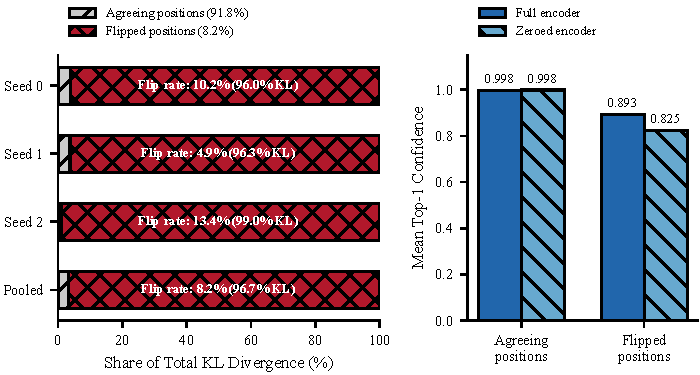
\includegraphics[width=0.80\textwidth]{figures/fig2_ablation_kl.pdf}
\caption{\textbf{Left:} share of total ablation KL contributed by agreeing versus
argmax-flipping decoding steps, per seed and pooled. The bars encode share of KL; the
percentages in the legend are share of \emph{steps}. Flipped steps are 8.2\% of steps but carry
96.7\% of the divergence. \textbf{Right:} mean top-1 confidence at agreeing and flipped
positions, with the full and zeroed encoder. Agreeing positions are pinned at 0.998 under both;
flipped positions remain high but not pinned.}
\label{fig:ablation}
\end{figure}

\paragraph{Two distinct interventions.} This section zeroes the encoder output.
Section~\ref{sec:position} uses blank white images, where the encoder still runs and produces
features of blankness. Zeroing asks whether the cross-attention pathway carries usable signal
at all; a blank image asks whether the model distinguishes content from its absence. We keep
them labelled separately.

\section{Mechanism II: Teacher-Forced Likelihood and the Position Profile}
\label{sec:position}

Max-softmax over a model's own greedily generated tokens is upward-biased by construction. We
therefore also compute teacher-forced log-likelihood of the ground-truth sequence,
conditioning on true preceding tokens and recording the probability assigned to the true next
token regardless of whether the model would have chosen it. Whole-sequence means are $-1.783$
(SD 1.274, $n=180$) on real input and $-1.751$ (SD 1.280, $n=180$) on blank, with mean
predictive entropy 0.0207 and 0.0251 respectively.

\paragraph{The two measures disagree in sign, and we spin neither.} Ground-truth likelihood is
marginally higher on blank, contrary to what grounded confidence predicts. Predictive entropy
is also higher on blank, meaning slightly less certain, which is exactly what grounded
confidence predicts. Both differences are negligible against their dispersions: 0.032 against
SDs near 1.27, and 0.004 against SDs near 0.017. Neither measure detects a difference between
real and blank, and the nominal signs should not be interpreted. The two estimators are also
not independent: both derive from the same softmax, differing in whether the conditioning
prefix is self-generated or ground truth.

\paragraph{Where the ground truth wins.} The ground-truth token is the model's argmax at 90.4\%
of positions on real input and 90.1\% on blank, with a mean peak probability of 0.9983 and
0.9982 at those positions, consistent with the reported entropy. Broken out by position:
\textbf{0\% at position 0}, on 0 of 180 sequences, under both conditions; 92.6\% (real) versus
92.3\% (blank) thereafter. That split is the shape of the whole result.

\begin{table}[h]
\small
\centering
\caption{Mean $\log p(\mathrm{GT})$ by generation position, against $n$-gram grapheme language
model references fitted on the same 2{,}491 training lines (evaluation strings excluded,
add-$\alpha$ smoothing with $\alpha = 0.01$) and evaluated \emph{within the same position
buckets}, so model and reference are position-matched. The $n$-gram models never see an image.
Token counts are over the 60 evaluation strings; instrument figures pool the same strings across
three seeds. Uniform over $|V|\approx367$ is $-5.91$.}
\label{tab:position}
\setlength{\tabcolsep}{4pt}
\begin{tabular}{lrrr@{\hskip 12pt}rrrrr}
\toprule
 & & \multicolumn{2}{c}{Instrument} & \multicolumn{5}{c}{Position-matched $n$-gram reference} \\
\cmidrule(lr){3-4}\cmidrule(l){5-9}
Positions & $n$ tok. & Real & Blank & 1-gram & 2-gram & 3-gram & 4-gram & 5-gram \\
\midrule
0      & 60  & $\mathbf{-24.54}$ & $-23.48$ & $-5.92$ & $-4.73$ & $-4.73$ & $-4.73$ & $-4.73$ \\
1      & 60  & $\mathbf{-8.12}$  & $-8.63$  & $-5.08$ & $-1.38$ & $-1.14$ & $-1.14$ & $-1.14$ \\
2--9   & 480 & $-0.48$ & $-0.41$ & $-4.11$ & $-2.25$ & $-0.88$ & $-0.38$ & $-0.31$ \\
10--19 & 598 & $-0.15$ & $-0.16$ & $-4.18$ & $-2.34$ & $-1.06$ & $-0.45$ & $-0.26$ \\
20--39 & 851 & $-0.27$ & $-0.28$ & $-4.13$ & $-2.24$ & $-0.98$ & $-0.43$ & $-0.20$ \\
40+    & 348 & $\mathbf{-6.12}$  & $-6.28$  & $-4.17$ & $-2.28$ & $-0.99$ & $-0.40$ & $-0.18$ \\
\bottomrule
\end{tabular}
\end{table}

\begin{figure}[h]
\centering

\includegraphics[width=0.84\textwidth]{figures/fig1_position_dissociation.pdf}
\caption{The dissociation. \textbf{Top:} mean $\log p(\mathrm{GT})$ against generation
position, real and blank overlaid. The horizontal reference lines drawn here are
\emph{whole-tail} $n$-gram means (trigram $-0.99$, 4-gram $-0.44$, 5-gram $-0.26$) computed
over all positions $\geq 1$; Table~\ref{tab:position} gives the position-matched references
that the argument in this section uses, and those differ per bucket. Uniform is $-5.91$.
The inset zooms positions 2--39 to separate the 4-gram and 5-gram references, and the
rightmost point aggregates positions 40 and beyond and is a categorical bin rather than a position on the continuous axis. The vertical axis of the top
panel is symmetric-log and therefore non-uniform: the interval from $-25$ to $-10$ occupies
comparable space to the interval from $-1$ to $0$, which compresses the region containing the
position-0 collapse. \textbf{Bottom:} self-generated max-softmax confidence at the same
positions, axis clipped to $[0.5, 1.0]$. Correctness
collapses at positions 0--1 while confidence does not, and both curves are near-identical
between real and blank input.}
\label{fig:position}
\end{figure}

Five observations, in order of importance.

\paragraph{1. Position 0 is far below a text-only baseline, not merely uncertain.} The geometric mean
probability assigned to the correct first symbol is $2.2\times10^{-11}$ on real images and
$6.3\times10^{-11}$ on blank. The model is not undecided at position 0; it is
near-deterministically committed to a specific wrong symbol, identically whether the image
contains text or nothing. We report the geometric mean because the arithmetic mean of
$p(\mathrm{GT})$ is dominated by a small number of less-severe cases and is not representative
of the distribution; Appendix~\ref{app:pos0} gives the per-seed figures and the histogram.

We deliberately do not anchor this on the uniform value of $2.725\times10^{-3}$. Self-generated
max-softmax at position~0 is 0.902 (next paragraph), so the position-0 distribution is nowhere
near uniform, and in a distribution that peaked almost any non-argmax symbol falls orders of
magnitude below $1/|V|$. A comparison against uniform would therefore partly measure the
sharpness of the softmax rather than a disfavouring of the truth specifically.

The position-matched $n$-gram references in Table~\ref{tab:position} supply a null that is not
subject to this objection, because both sides of the comparison are $p(\mathrm{GT})$. A
grapheme $n$-gram model fitted on the same training corpus, which never sees an image, assigns
the correct first symbol $-4.73$ nats at position~0 (identical for orders two through five,
since with no prefix they all reduce to the marginal over sequence-initial symbols). The
instrument assigns it $-24.54$. That is a gap of 19.8 nats, or more than eight orders of
magnitude, \emph{below a text-only baseline}. The model is not merely failing to use the image
at position~0; it is placing the correct first symbol far lower than a model that has only ever
seen text. We regard this, rather than the comparison against uniform, as the defensible form
of the claim.

Two scale-free quantities would sharpen it further and neither is computed here: the
probability the model assigns at position~0 to an arbitrary \emph{wrong} symbol, and the rank
of the ground-truth symbol in that distribution. Both are listed in Section~\ref{sec:lim}.

\paragraph{2. Confidence at that position is near ceiling.} Self-generated max-softmax at
position 0 is 0.902 pooled on real input and 0.895 on blank. Position 0 is therefore the point
of maximal confidence and minimal correctness, at the one generation step where vision is the
only possible information source. Per seed, real: 0.884 / 0.906 / 0.916; blank: 0.9999 / 0.898
/ 0.787. The blank column is not stable across seeds and its pooled value should not be quoted
alone.

\paragraph{3. Position 1 is also far below the text-only baseline.} At $-8.12$ and $-8.63$ the
second generated symbol sits 7.0 nats (real) and 7.5 nats (blank) below the best
position-matched $n$-gram reference for that position ($-1.14$). The failure is not confined to
a single step; recovery begins at position 2.

\paragraph{4. In the middle of the sequence the model is comparable to a high-order grapheme
prior.} Against position-matched references (Table~\ref{tab:position}), positions 2--9
($-0.48$) sit between the trigram ($-0.88$) and 4-gram ($-0.38$) references; positions 10--19
($-0.15$) are slightly \emph{better} than the 5-gram reference ($-0.26$); positions 20--39
($-0.27$) sit between the 4-gram and 5-gram references. So mid-sequence the instrument is in
the same band as a 4- to 5-gram grapheme prior, occasionally above it, and it gets there
without reference to the image, since the blank column matches the real column at every bucket.

One property of this reference deserves stating. The training text is drawn from the same
GlotOCR Hindi string pool that the evaluation strings come from, resampled into synthetic pages,
and the $n$-gram models are fitted on that pool. A 5-gram grapheme model reaching $-0.18$
(roughly 0.84 per token) on about 2{,}500 lines implies that contexts recur heavily, which
resampling produces by construction. The 5-gram reference is therefore closer to a memorisation
baseline than to a generic language prior. This cuts in the direction of our claim rather than
against it, since matching a memorising model mid-sequence is a stronger indictment than
matching a generic one, but the comparison should be read with that in mind. The same
repetition may also bound the 18.3\% line accuracy reported in Section~\ref{sec:works}.

We stop short of the exclusive claim. Matched mean log-likelihood does not establish that two
predictive distributions agree, and establishing that the decoder is a high-order $n$-gram
model \emph{and nothing more} would require a distributional comparison, for instance
per-position $\mathrm{KL}$ between the model and the 5-gram reference together with the rate at
which their argmaxes coincide. The committed probe outputs record $p(\mathrm{GT})$ and entropy
per step but not the full softmax, so that comparison is not available here.

\paragraph{5. Outside that band the model is far worse than a text-only baseline.} The
position-matched view makes the shape of the failure precise, and it is not the shape a
low-order-$n$-gram account predicts. At position~0 the instrument is 19.8 nats below the best
$n$-gram reference; at position~1 it is 7.0 nats below; and beyond position~39 it is 5.9 nats
below the 5-gram reference, on 348 evaluation tokens. The $n$-gram baselines are
essentially flat across buckets (the 5-gram reference moves only from $-0.31$ to $-0.18$), so
the instrument's profile is not tracking any property of the text. It matches a text-only prior
in the middle of the sequence and collapses far beneath one at both ends. We place limited
weight on the 40+ bucket, since sequences reaching that length are a selected minority, but the
position-0 and position-1 gaps rest on all 180 sequences.

\section{When the Confidence Signal Does Work}
\label{sec:works}

A purely negative result would leave open the possibility that this model's confidence head is
simply broken. It is not, and the contrast is informative.

\begin{table}[h]
\small
\centering
\caption{Confidence as a predictor of correctness across evaluation regimes; $n$ pools 100 or 60
images over three seeds. AUROC is against line-level exact correctness except in the final row,
which uses a median split on grapheme CER because exact accuracy is identically zero. On the
flattened and inverted sets at most one line per seed is exactly correct, so AUROC there is
computed on one or zero positive cases and carries no information; we mark it uninformative
rather than reporting the value.}
\label{tab:auroc}
\setlength{\tabcolsep}{4pt}
\begin{tabular}{lrccc}
\toprule
Evaluation set & $n$ & Line acc. & AUROC & Spearman (conf, CER) \\
\midrule
Synthetic, natural exposure        & 300 & 0.183 & \textbf{0.838} & $-0.40$ \\
Synthetic, flattened / inverted    & 300 / 300 & 0.003 / 0.007 & uninformative & $\approx 0$ \\
Real Hindi scans                   & 180 & 0.000 & undefined & $-0.15$ \\
Real Hindi scans, median CER split & 180 & ---   & 0.57 & --- \\
\bottomrule
\end{tabular}
\end{table}

\begin{figure}[t]
\centering

\includegraphics[width=0.78\textwidth]{figures/fig4_regime_contrast.pdf}
\caption{\textbf{Left:} confidence as a ranker of correctness in two regimes. The synthetic
curve is against line-level exact correctness; the real-scan curve is against a median split on
grapheme CER, because exact accuracy on real scans is identically zero and the AUROC against it
is undefined (Table~\ref{tab:auroc}). The two curves therefore answer slightly different
questions and should not be read as a like-for-like comparison. \textbf{Right:} reliability
diagram on synthetic natural lines, equal-mass confidence deciles. Confidence is near unity in
every decile while accuracy is not, so the model discriminates without being calibrated.}
\label{fig:regime}
\end{figure}

On synthetic in-distribution lines, where the model reads well enough to get 18.3\% of lines
exactly right, confidence ranks correct transcriptions above incorrect ones at AUROC 0.838.
That is a working discrimination signal (per seed 0.763, 0.924, 0.832; bootstrap 95\% interval
[0.771, 0.902]), and it is nonetheless badly calibrated: mean confidence in that regime is 0.994
against 18.3\% accuracy, giving an expected calibration error of 0.811 over ten equal-mass
bins. Discrimination and calibration
come apart cleanly here, and only the former survives. On real scans, where accuracy is
zero, a graded substitute gives 0.57, near chance. Mean confidence across the three synthetic
exposure conditions also varies substantially, at 0.994 (natural), 0.600 (flattened) and 0.461
(inverted), tracking the accuracy drop in those conditions.

Taking this together with Sections~\ref{sec:cer}--\ref{sec:position}, the reading best
supported by the evidence is that \textbf{the model's confidence responds to properties of the
text it is generating, not to whether the image supports that text.} It falls when the target
text has unfamiliar statistics. It does not fall when the image is blank, unreadable, or in a
script the model has never seen, because in those cases the decoder still produces fluent,
familiar Devanagari. We offer this as an interpretation consistent with what we measured, not
as a demonstrated mechanism.

\section{Limitations and Future Work}
\label{sec:lim}

\paragraph{No positive control; this is the central limitation.} We have no model with
demonstrated Devanagari reading ability on which the position-0 measurement returns a different
answer. Without that contrast the measurement has no established dynamic range, and a reader
cannot distinguish a working instrument from a broken one on this evidence alone. The control
is already available and we did not use it: Surya, one of the engines in
Table~\ref{tab:tier1}, attains 46.8\% exact match on real Indic scans including Devanagari, is
an open-weight encoder--decoder architecture in the same family as our instrument, and therefore
admits position-resolved teacher-forced $\log p(\mathrm{GT})$, encoder zeroing and blank-input
evaluation on exactly the protocol used here. Running the full suite on it is the next
experiment rather than an optional extension. Broader benchmarks of real-scan Devanagari
competence \citep{singh2026devanagari} identify stronger candidates, though the top-scoring
systems there are closed and do not expose per-step likelihoods.

\paragraph{Two measurements the position-0 claim needs.} The comparison in
Section~\ref{sec:position} is between $p(\mathrm{GT})$ and the model's own selected symbol,
which is sound, but two scale-free quantities would make it decisive and neither is computed
here. First, the probability the model assigns at position~0 to an arbitrary non-argmax symbol:
if that is orders of magnitude above $p(\mathrm{GT})$, the collapse is specific to the correct
symbol; if it is comparable, the finding reduces to the position-0 softmax being extremely
peaked with the truth outside the peak, which is a weaker and different statement. Second, the
rank of the ground-truth symbol among the 367 candidates, which is invariant to softmax
temperature and directly comparable across models, including against the control above. Both
are single forward passes over the existing checkpoints.

\paragraph{Three further interventions we consider necessary.} First, \emph{mismatched
pairing}: teacher-forced $\log p(\mathrm{GT})$ under a derangement of the image pool, so each
ground-truth string is scored against a different real image. A blank page is a degenerate
input, so ``blank equals real'' is weaker evidence than ``wrong real image equals right real
image'' would be, and the latter would remove the degeneracy confound of
Section~\ref{sec:degeneracy} entirely. Second, \emph{cross-attention contribution norms},
$\|\text{cross-attn out}\|/\|\text{residual}\|$ per decoder layer, which would convert the
behavioural claim that the model ignores the encoder into a direct measurement of how much
signal that pathway carries. Third, \emph{Gaussian-noise and patch-scrambled inputs}, testing
whether the model responds to visual variation of any kind rather than only to the blank
versus real contrast; these are also what would separate visual bypass from the domain-shift
explanation raised in Section~\ref{sec:cer}. A fourth would make Section~\ref{sec:position}'s
$n$-gram claim exclusive rather than merely consistent: per-position $\mathrm{KL}$ between the
model and the 5-gram reference, and the rate at which their argmaxes coincide. This requires
retaining the full per-step softmax, which the committed probe outputs do not. All four, together with the positive control above, are inference-only measurements requiring
no further training. They were scoped out of the present phase by
available compute rather than by design, and the probe implementations are released with the
code.

\paragraph{Scale and generality.} One model of approximately 19.6M parameters, one training
script for the mechanistic experiments. We make no claim about production OCR systems. A
separate attempt to use TrOCR-base-printed as an external comparison found mean confidence
0.42 on its own in-domain English text, far below this instrument's near-ceiling regime; that
is an operating-regime mismatch rather than a failed replication, and it does not serve as a
control.

\paragraph{Code and data.} The instrument, the renderer, all probe implementations and the
committed probe outputs from which every number in this paper is computed are available at
\url{https://github.com/Adya6714/vlm-ocr-eval}.

\paragraph{Metric choice.} Line-level exact match is uninformative here and is used only in
Section~\ref{sec:works}, where the comparison is between regimes rather than between
conditions. Grapheme CER is what Section~\ref{sec:cer} reports.

\paragraph{The exposure-versus-complexity question is unanswered.} We believe the fix is to
abandon distributional-target synthesis in favour of subsampling real, naturally learnable
sentences to bias exposure, accepting weaker distributional control in exchange for text that
remains learnable.

\paragraph{Novelty relative to prior work.} Two things in this paper are not new and we do not
present them as such. That a multimodal model's confidence is insensitive to visual ablation is
established \citep{khanmohammadi2026bicr}. That visual reliance declines across generation
positions, and that the first generated token carries the most visual evidence, are established
too \citep{favero2024m3id,ha2026flb}, on models that read their inputs and as the basis for
decoding methods rather than as objects of study.

What we add is the boundary case and one decomposition. Prior work characterises the
\emph{gradient} of visual reliance in grounded models; we characterise the profile when there
is no visual reliance for it to decline from, and find that position~0 is not merely the least
language-supported position but one where the ground-truth symbol is never the argmax across
180 sequences, while self-reported confidence there is at its maximum. Separately, the
shape-versus-peak decomposition in Section~\ref{sec:ablation} is a sharper statement than
``confidence fails to detect ungroundedness'': ablation moves \emph{which} token holds the
peak without moving \emph{that} there is a near-unit peak, and the deployed scalar is the
component it leaves untouched. The within-instrument regime contrast in
Section~\ref{sec:works} is what keeps this from being a purely negative result.

\section{Discussion and Conclusion}

Three implications follow from the position profile, if it holds under a positive control.
Visual dependence in autoregressive transcription is concentrated at the start of the
sequence: positions 2 to 39 are recoverable from the prefix alone at 62--86\% per-token
likelihood, in the band of a position-matched 4- to 5-gram grapheme prior, and near-identically
so with no image at all. Any confidence
score averaged uniformly over the generated sequence therefore averages the one
vision-dependent position against many that are not, diluting exactly the signal a gating
system needs; confidence measures for transcription should weight early positions. The
diagnosis is also cheap: two forward passes and ground-truth text give the position profile,
with no probe training and no auxiliary labels. Interpreting it against a reference model is a
separate requirement, and one we have not met (Section~\ref{sec:lim}). Where probe-based
approaches \citep{khanmohammadi2026bicr,yao2025abstain,kogilathota2026halp} detect
ungroundedness by learning it, the position-0 test asks a structural question with a known
answer under grounding. And the failure mode is a training pathology that standard monitoring
would not catch: a model in this state converges, produces fluent in-script output, and
reports mean confidence of 0.99.

We audited a small, fully exposure-controlled document OCR model and found that it does not
read real document images. We localised the failure to the start of the generated sequence,
where the ground-truth symbol is never the model's argmax across 180 sequences and receives a
geometric mean probability of order $10^{-11}$, more than eight orders of magnitude below what a
text-only $n$-gram model fitted on the same corpus assigns it, identically with and without
visual content, while the model's own selected symbol at that position receives 0.90. We showed that deleting the
encoder alters the output distribution's shape substantially while leaving its peak near
unity, so that the quantity read as confidence is close to invariant under precisely the
intervention that removes visual information. And we showed that the same confidence signal
does discriminate correctness in a regime where the model reads, locating the failure in the
relationship between confidence and vision rather than in the confidence head itself.

\bibliographystyle{plainnat}
\bibliography{refs}

\appendix

\section{A Retracted Single-Seed Result}
\label{app:retraction}

An earlier analysis using only seed 0 reported a statistically significant confidence
difference on the Perso-Arabic condition relative to in-distribution Hindi ($|z| = 2.54$). It
did not replicate: at seed 1, Hindi confidence (0.9897) exceeded Perso-Arabic (0.9894),
reversing the original direction. We retract the claim in full and report it as the failure
mode that motivated the three-seed design.

\section{Position-0 Likelihood Distribution}
\label{app:pos0}

Per-seed geometric means of $p(\mathrm{GT})$ at position 0 are $2.05\times10^{-10}$ /
$1.35\times10^{-11}$ / $3.88\times10^{-12}$ (real) and $9.32\times10^{-10}$ /
$3.13\times10^{-11}$ / $8.70\times10^{-12}$ (blank). The effect is present independently at
every seed and spans two orders of magnitude across seeds, so per-seed values rather than the
pooled geometric mean should be used when comparing against another model.

A geometric mean can be driven by a minority of extreme cases, so we report the distribution.
Pooled over 180 sequences, the median $p(\mathrm{GT})$ at position 0 is $9.5\times10^{-15}$
(real) and $3.7\times10^{-13}$ (blank); the arithmetic means are $2.67\times10^{-3}$ and
$1.51\times10^{-3}$, close to uniform, but they are set by a handful of sequences. Only
2.8\% of real sequences (5 of 180) and 3.3\% of blank sequences (6 of 180) assign the correct
first symbol more probability than uniform.

\begin{table}[h]
\small
\centering
\caption{Histogram of $\log p(\mathrm{GT})$ at position 0, pooled over three seeds.}
\begin{tabular}{lrrrr}
\toprule
Bin ($\log p$) & Real count & Real \% & Blank count & Blank \% \\
\midrule
$< -25$        & 126 & 70.0\% & 115 & 63.9\% \\
$[-25, -20)$   & 24  & 13.3\% & 25  & 13.9\% \\
$[-20, -15)$   & 14  & 7.8\%  & 13  & 7.2\%  \\
$[-15, -10)$   & 8   & 4.4\%  & 13  & 7.2\%  \\
$[-10, -5)$    & 6   & 3.3\%  & 10  & 5.6\%  \\
$[-5, 0]$      & 2   & 1.1\%  & 4   & 2.2\%  \\
\bottomrule
\end{tabular}
\end{table}

Seventy percent of real sequences place $\log p(\mathrm{GT}) < -25$ at position 0. The
collapse is a property of the distribution, not of its summary.

\section{Paired Tests and Bootstrap Intervals}
\label{app:stats}

Because the same 60 image identifiers appear under every condition, we use paired rather than
unpaired tests. Per-seed Wilcoxon signed-rank on grapheme CER (real minus blank) gives
$+0.180$ ($p = 1.4\times10^{-6}$), $+0.088$ ($p = 0.106$) and $-0.159$ ($p = 0.015$) at seeds
0, 1 and 2. The sign reverses at seed 2. Pooled unclustered the difference is $+0.036$
($p = 0.025$); clustered by seed it is not significant ($t = 0.257$, $p = 0.822$). For mean
confidence the pooled difference is $+0.0016$ ($t = 0.505$, $p = 0.664$).

Seed-clustered bootstrap intervals (2{,}000 replicates, images resampled within seed):
grapheme CER 0.9855 [0.9406, 1.0347] real and 0.9491 [0.9053, 0.9911] blank; mean confidence
0.9873 [0.9852, 0.9892] real, 0.9857 [0.9838, 0.9874] blank, 0.9857 [0.9843, 0.9871] Ol Chiki
and 0.9894 [0.9871, 0.9916] Perso-Arabic; position-0 geometric mean $p(\mathrm{GT})$
$2.20\times10^{-11}$ [$1.04\times10^{-11}$, $5.29\times10^{-11}$] real; AUROC 0.838
[0.771, 0.902] on synthetic natural and 0.570 [0.491, 0.650] on real scans.

\section{Training and Evaluation Configuration}
\label{app:config}

\paragraph{Architecture.} Vision Transformer encoder, 6 layers, $d_{\text{model}} = 320$, 5
heads, MLP ratio 4, dropout 0.1, sinusoidal position encodings, single grayscale input channel.
Autoregressive decoder, 5 layers, $d_{\text{model}} = 384$, 6 heads, MLP ratio 4, dropout 0.1,
learned position encodings, embedding and output head tied. Patch size 14. Total parameters
19{,}607{,}104 at $|V| = 367$. The vocabulary is built from the run's own manifest with a
minimum grapheme frequency of 5.

\paragraph{Training data.} Rendered Hindi line crops in the \texttt{natural} glyph-frequency
mode, 2{,}538 lines; the flattened and inverted modes contain 2{,}707 and 2{,}872 lines. Source
text is ground-truth strings from GlotOCR Hindi \citep{kargaran2026glotocr}, resampled into
synthetic pages. Fonts are selected as the first available among Kohinoor, Sangam, ITF or Noto
Sans Devanagari; the specific font file used for the training run was not recorded. No
augmentation is applied at training time: crops are loaded grayscale, divided by 255 and
white-padded. Line crops are rendered at height 70 px (five patches) with variable width padded
per batch to a multiple of the patch size.

\paragraph{Optimisation.} AdamW, learning rate $3\times10^{-4}$ held constant with no schedule,
batch size 32, 5{,}000 steps, fp16 mixed precision. The checkpoint used throughout is the final
step of the run; there is no validation-loss selection. Three seeds were trained under
identical settings. Wall-clock was not recorded.

\paragraph{Evaluation data.} Real evaluation images are resized to height 70 preserving aspect
ratio (Lanczos); their native resolution and scanning conditions were not recorded. The
model-side evaluation uses 60 real Hindi rows in plain and degraded variants, 100 Ol Chiki rows
and 20 Perso-Arabic rows, each under three seeds. Grapheme-cluster segmentation for every CER
in this paper uses the \texttt{regex} library's \texttt{{\textbackslash}X} operator.

\paragraph{Scope of the engine study.} The counts in Table~\ref{tab:tier1} are prediction rows
pooled over three engines, four languages (Hindi, Bengali, Santhali, Kashmiri) and two image
variants, scored on full strings. They are not the same evaluation set as the model-side
results and the overlap between the two was not recorded.

\section{Sequence Lengths}
\label{app:lengths}

Mean and median generated grapheme lengths are 27.96 / 28.0 (real Hindi), 31.39 / 29.0
(blank), 28.28 / 29.0 (Ol Chiki) and 33.40 / 35.0 (Perso-Arabic), $n$ as in
Table~\ref{tab:cer}. Blank generations are not shorter than real ones, which rules out
truncation as the explanation for the CER ordering in Section~\ref{sec:cer} and leaves
repetition, documented in Section~\ref{sec:degeneracy}, as the operative mechanism.

\end{document}
